\section{Approach}
\label{sec:pagestyle}
\begin{figure*}[t]
  \centering
  \centerline{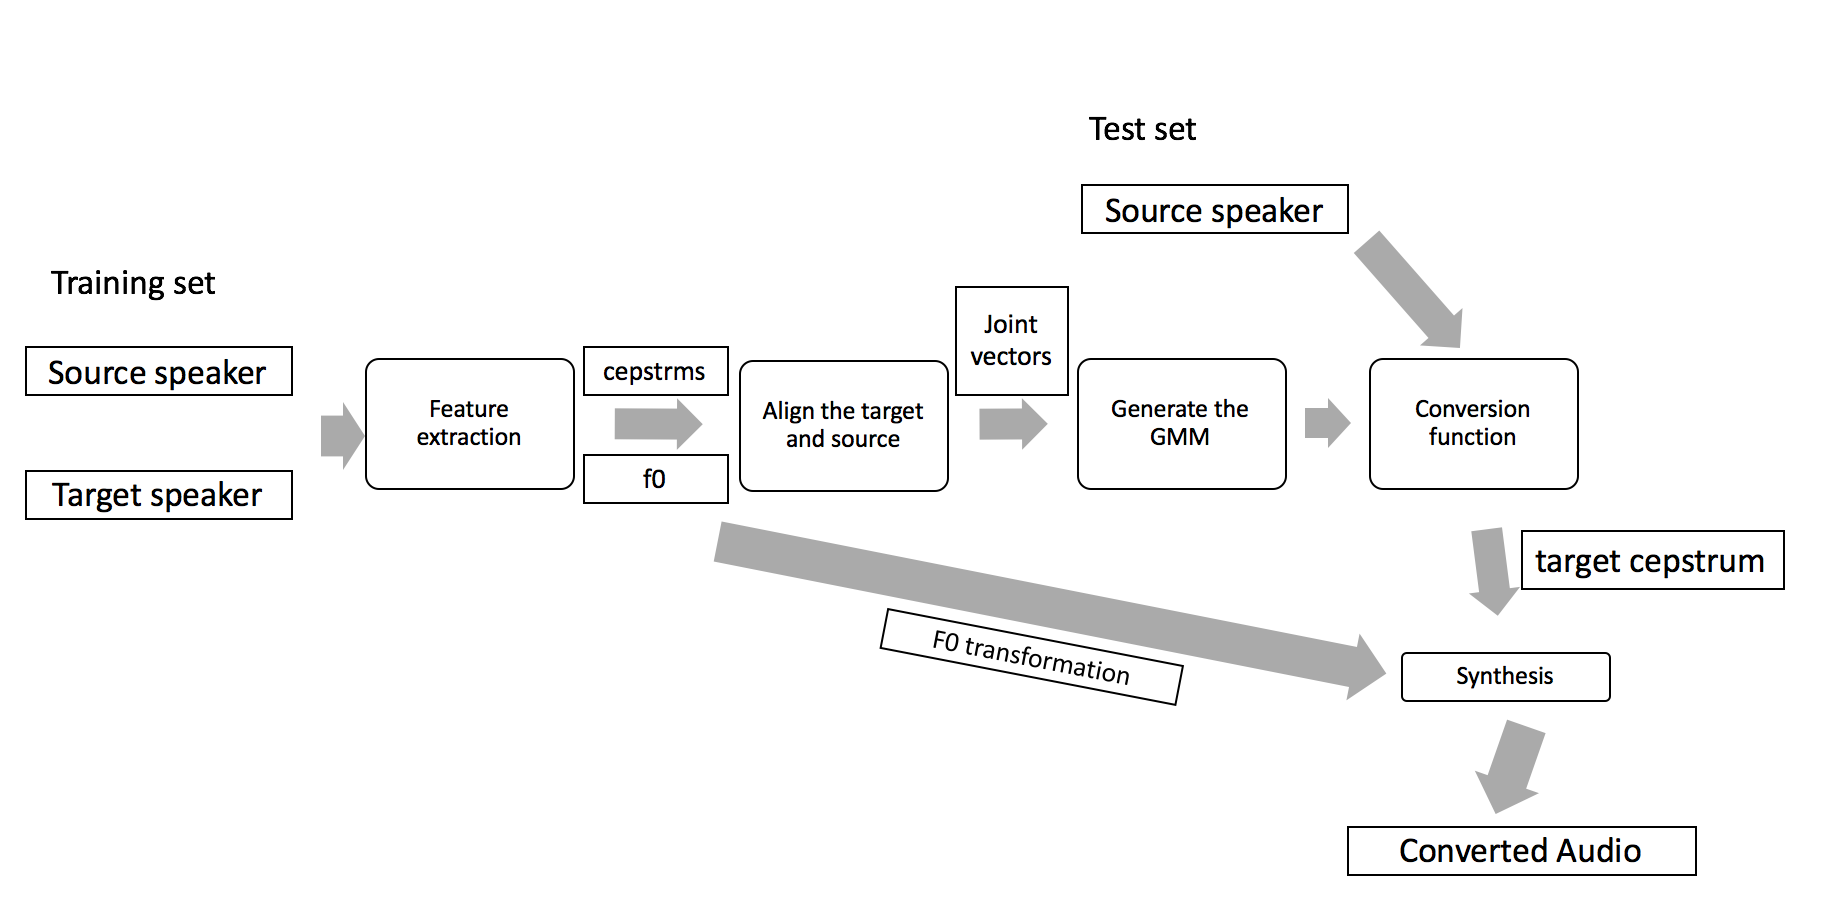
\includegraphics[width=\linewidth]{image11}}
%  \vspace{2.0cm}
\caption{The algorithm flowchart}
\label{fig:algorithm}
%
\end{figure*}

Based on the complexity of this field and the duration of our project, we chose to implement an algorithm based on a foundational paper in the field. Specifically, Stylianou's foundational work\cite{stylianou1998continuous}, on which more advanced voice conversion technology is based. In this section, we will cover in detail our approach of the feature extraction for cepstrums and fundamental frequency, the alignment of the source and target feature using dynamic time warping, and the use of GMM in training with 2 different conversion functions. 

\subsection{Dataset and Software}We used the dataset from VCC2016\cite{toda2016voice}, which contains 5 source speakers and 5 target speakers. Each speaker utters the same sentence set of 162 sentences. We selected 160 sentences from one source speaker and one sentence speaker. Of the 160 pairs of sentences,  150 pairs of them are used for training and 10 for testing. The sampling rate is 16 kHz, and stored in 16-bit format. Various python libraries were used for the purpose of this project including \texttt{dtw}, \texttt{pyworld}, \texttt{pysptk}, and \texttt{sklearn}.

\subsection{Feature Extraction}
Using a time step of $5ms$, we extracted 25 mel-frequency cepstrums from each time step.
\subsection{Alignment}
We implemented the Dynamic Time Warping(DTW) method mentioned in the background section to generate the aligned features for the source and target features.
\subsection{GMM}
The basic idea is to train GMMs for the joint vector features for source and target spectral features. EM algorithm with Maximum Likelihood Estimation iteratively generates a GMM for the aligned features of the source and target. 
Once we have the GMMs models, the next step is to use GMMs for converting source features to target features. The GMM conversion function deserves special treatment due to its complexity. The primary component of the conversion function is a conditional probability built on the GMM. From the GMM, it is possible to calculate the probability of a target cepstrum given the source speech cepstrum. 
\begin{align*}
    p(x) = \sum_{i=1}^m \alpha_i N(x;\mu_i,\Sigma_i)
\end{align*}

The paper by Stylianou\cite{stylianou1998continuous} proposes and compares three different conversion methods: Full, Diagonal, and VQ Conversion. In our work, we implemented Full and VQ conversion for comparison. Each class in the GMM model is defined by its parameters: mean and variance. As a result, different posteriori conversion functions can be used to convert target to source based on the GMM components and their parameters. VQ only considers only the mean target vector, whereas Full also considers the cross-covariance matrix of source and target vectors, which acts as a correction term to achieve the minimum mean-squared error.
\begin{align*}
    \text{VQ Conversion:}\\
    F(x_t) &= \sum_{i=1}^m P(C_i|x_t)\nu_i \\
    \text{Full Conversion:}\\
    F(x_t) &= \sum_{i=1}^m P(C_i|x_t)[\nu_i + \Gamma_i\Sigma_i^{-1}(x_t-\mu_i)] \\
\end{align*}
Where $\nu$  is the mean target vector and $\Gamma$ is the cross-covariance matrix between source and target.
Since Full conversion is more complicated but is the more accurate model, the following table shows the comparison of the two conversion functions:
\begin{center}
    \begin{tabular}{ | c | c | c |}
    \hline
    Conversion & Performance & Computation \\\hline
    VQ & poor & simple\\ \hline
    Full & best & costly\\ \hline
    % Diagonal & better than VQ & better than Full\\ \hline
    \end{tabular}
\end{center}   
\subsection{Algorithm}
In conclusion, the algorithm can be described as follows and in Figure \ref{fig:algorithm}:
\begin{enumerate}
\item Calculate the Mel cepstrum
\item Align the target and source speaker's cepstrums
\item Generate the GMM on source and target training data
\item Convert a source cepstrum to the matching target cepstrum using the conversion function
\item Convert the cepstrum back to speech audio:
\begin{enumerate}
\item Convert the cepstrum to the frequency domain.
\item Match the average fundamental frequency to the target.
\item Convert the spectrogram back to the time domain.
\end{enumerate}
\end{enumerate}
